\subsection{Итеративный метод диаграммообразования}\label{sect:iterative-theory}

\subsubsection{Обзор существующих решений}

Идея поиска положения цели в систем радиолокации и радионавигации за счёт использования нескольких систем не нова. 
Так, например, радиосистемы посадки самолётов сантиметрового диапазона применяют два радиолокатора - азимутальный 
и угломестный. Каждый из этих радиолокаторов имеет узкую диаграмму направленности лишь в одной плоскости, и широкую в 
другой. Такой подход позволяет ускорить поиск цели. Местонахождение искомого летательного аппарата определяется в 
полярных координатах на пересечении этих ДН \cite{BakulevSosnovsky2005}.

\begin{figure}[H]
    \centering
    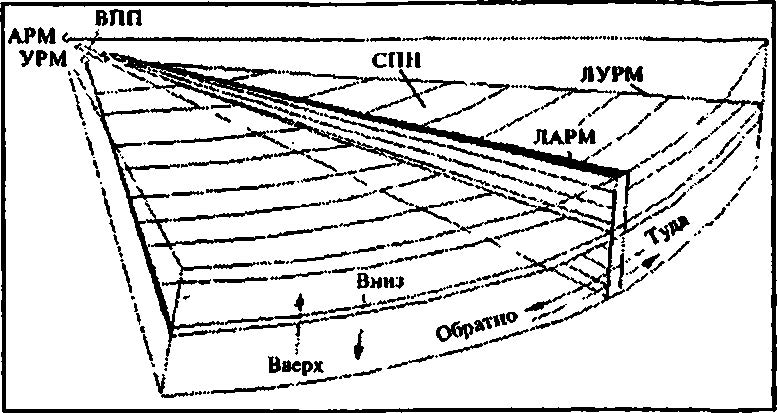
\includegraphics[width=0.8\textwidth,height=0.35\textheight,keepaspectratio]{cm-wave-plane-landing-system}
    \caption{Сектор пропорционального наведения АРМ и УРМ \cite{BakulevSosnovsky2005}}%
    \label{fig:cm-wave-plane-landing-system}
\end{figure}

Похожий подход применяют фазовые дальномерные РНС такие как РНС “Omega”. Для оценки нескольких областей поиска 
применяются сигналы на разных частотах - низкочастотный проводят грубую оценку и позволяют устранить 
неопределённость/многовариативность местоположения объекта, а высокочастотные уточняют местоположение внутри 
выбранной области \cite{BakulevSosnovsky2005}.

\begin{figure}[H]
    \centering
    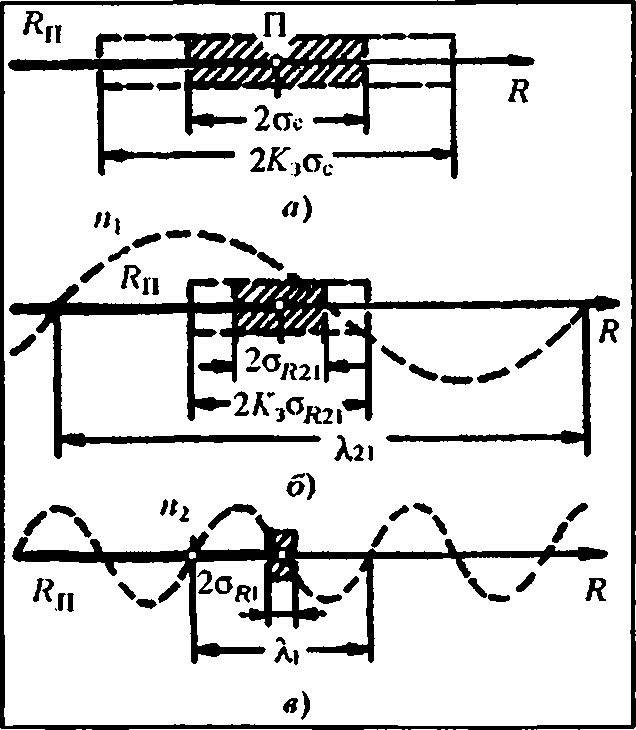
\includegraphics[width=0.8\textwidth,height=0.35\textheight,keepaspectratio]{phase-distance-measurment}
    \caption{Поиск местоположения на (а) грубой (б) средней и (в) точной шкалах \cite{BakulevSosnovsky2005}}%
    \label{fig:phase-distance-measurment}
\end{figure}

Более похожий на предлагаемый подход применяется в РЛС таких как “Воронеж” и “Небо-СВ”. В состав этих систем входит 
несколько АР разных диапазонов. Антенные решётки метрового диапазона проводят грубую оценку на больших дистанциях, 
а АР сантиметрового диапазона осуществляют точную оценку параметров цели и слежение.

\subsubsection{Описание метода}

Рассматриваемый метод предлагает использовать одни и те же данные по несколько раз в разных комбинациях для 
формирования итоговой ДН.

На Рисунке~\ref{fig:iterative-method-element-placing} показано расположение элементов в антенной решётке. Также для сравнения 
приведена эквидистантная решётка таких же размеров. Рассматриваемая решётка получена из эквидистантной путём 
удаления элементов на краях антенны. 

\begin{figure}[!ht]
    \centering
    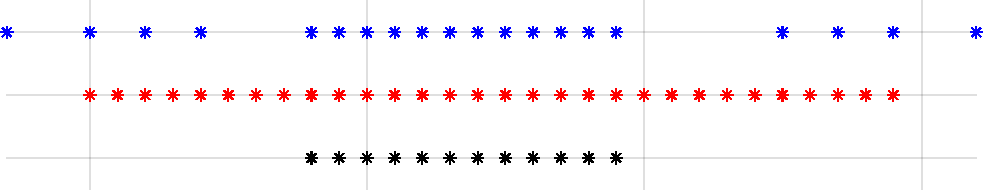
\includegraphics[width=0.8\textwidth,height=0.35\textheight,keepaspectratio]{iterative-method-element-placing}
    \caption{Расположение элементов в эквидистантной решётке (красный), рассматриваемой решётке (синий) и эквидистантной подрешётке (чёрный)}%
    \label{fig:iterative-method-element-placing}
\end{figure}

Формирование ДН данным методом разделено на следующие шаги:

\begin{enumerate}
    \item Проектирование разреженной антенной решётки
    
    За основу берётся модель эквидистантной антенной решётки, из которой удаляются элементы таким образом, что чем ближе к 
    краю будут расположены элементы, тем больше будет расстояние до следующего элемента. Затем к краям добавляются 
    два элемента, расстояние до них определяется тем же принципом.
    \item Принятый сигнал получается за счёт применения формирующих коэффициентов к двум решёткам - полной, т.е. ко 
    всем элементам разреженной решётки; краевым подрешёткам, т.е. ко всем кроме составляющих центральную подрешётку; 
    и к центральной подрешётке
    \item После того как сигналы в каналах будут умножены на соответствующие коэффициенты, проводится 
    свёртка полученных результатов и последующее сканирование
\end{enumerate}

В разделе~\ref{sect:iterative-modeling} проведено моделирование данного метода, приведены достоинства, недостатки и возможные пути развития.